\documentclass[mathserif,serif]{beamer}
\useoutertheme{infolines}
%\usepackage{tabularx}
%\usepackage{amsmath}

\title[Oral Presentation]{Search for chargino and neutralino production in final states with two same-sign leptons, jets and missing transverse momentum at $\sqrt{s} = 13$ TeV with the ATLAS detector}
\author[]
{
Samuel Lo \inst{1}
}
\institute[]
{
\inst{1}
The University of Hong Kong
}
\date[]{\today}

\newcommand\Wider[2][2em]{%
\makebox[\linewidth][c]{%
\begin{minipage}{\dimexpr\textwidth+#1\relax}
\raggedright
\centering#2
\end{minipage}%
}%
}

\begin{document}

\frame{\titlepage}
\frame{\tableofcontents}

\section{Introduction}
\begin{frame}
\begin{center}
\huge
Introduction
\end{center}
\end{frame}

\begin{frame}{Standard Model}
\begin{itemize}
\item Standard Model(SM) is the current mainstream theory to describe the electromagnetic force, weak force and strong force.
\end{itemize}

\begin{figure}
\centering
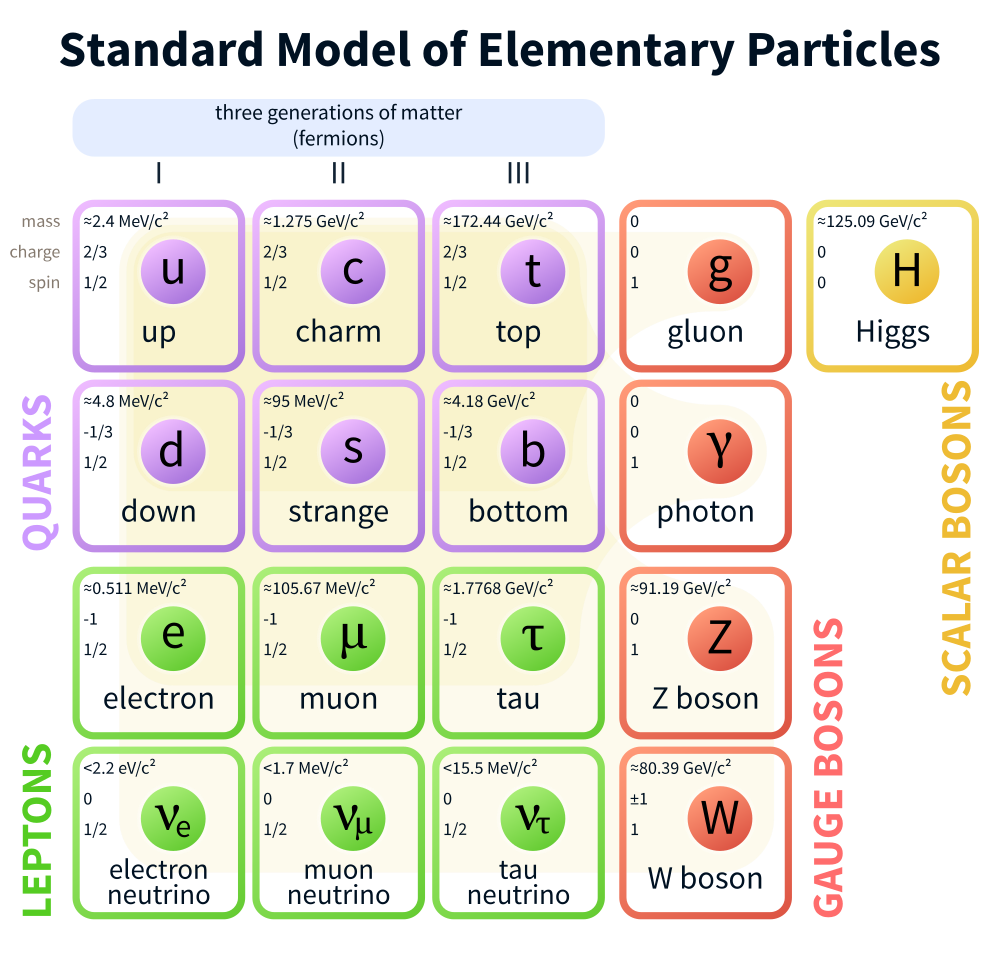
\includegraphics[width=0.5\textwidth]{data/photo/theory/SM_particles.png}
\caption{The table for all fundamental particles in SM.}
\end{figure}
\end{frame}

\begin{frame}{Standard Model}
\begin{columns}

\begin{column}{0.5\textwidth}
\begin{figure}
\centering
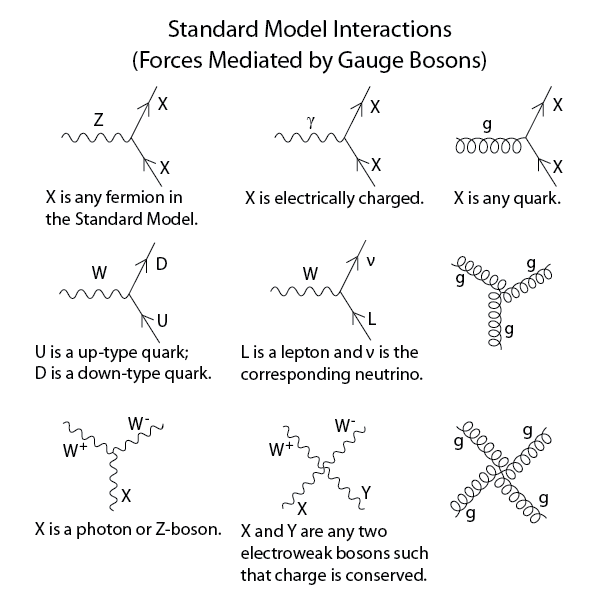
\includegraphics[width=\textwidth]{data/photo/theory/vertices_SM.png}
\caption{All allowed fundamental Feynman vertices in SM, except higgs-related vertices.}
\end{figure}

\end{column}

\begin{column}{0.5\textwidth}
\begin{figure}
\centering
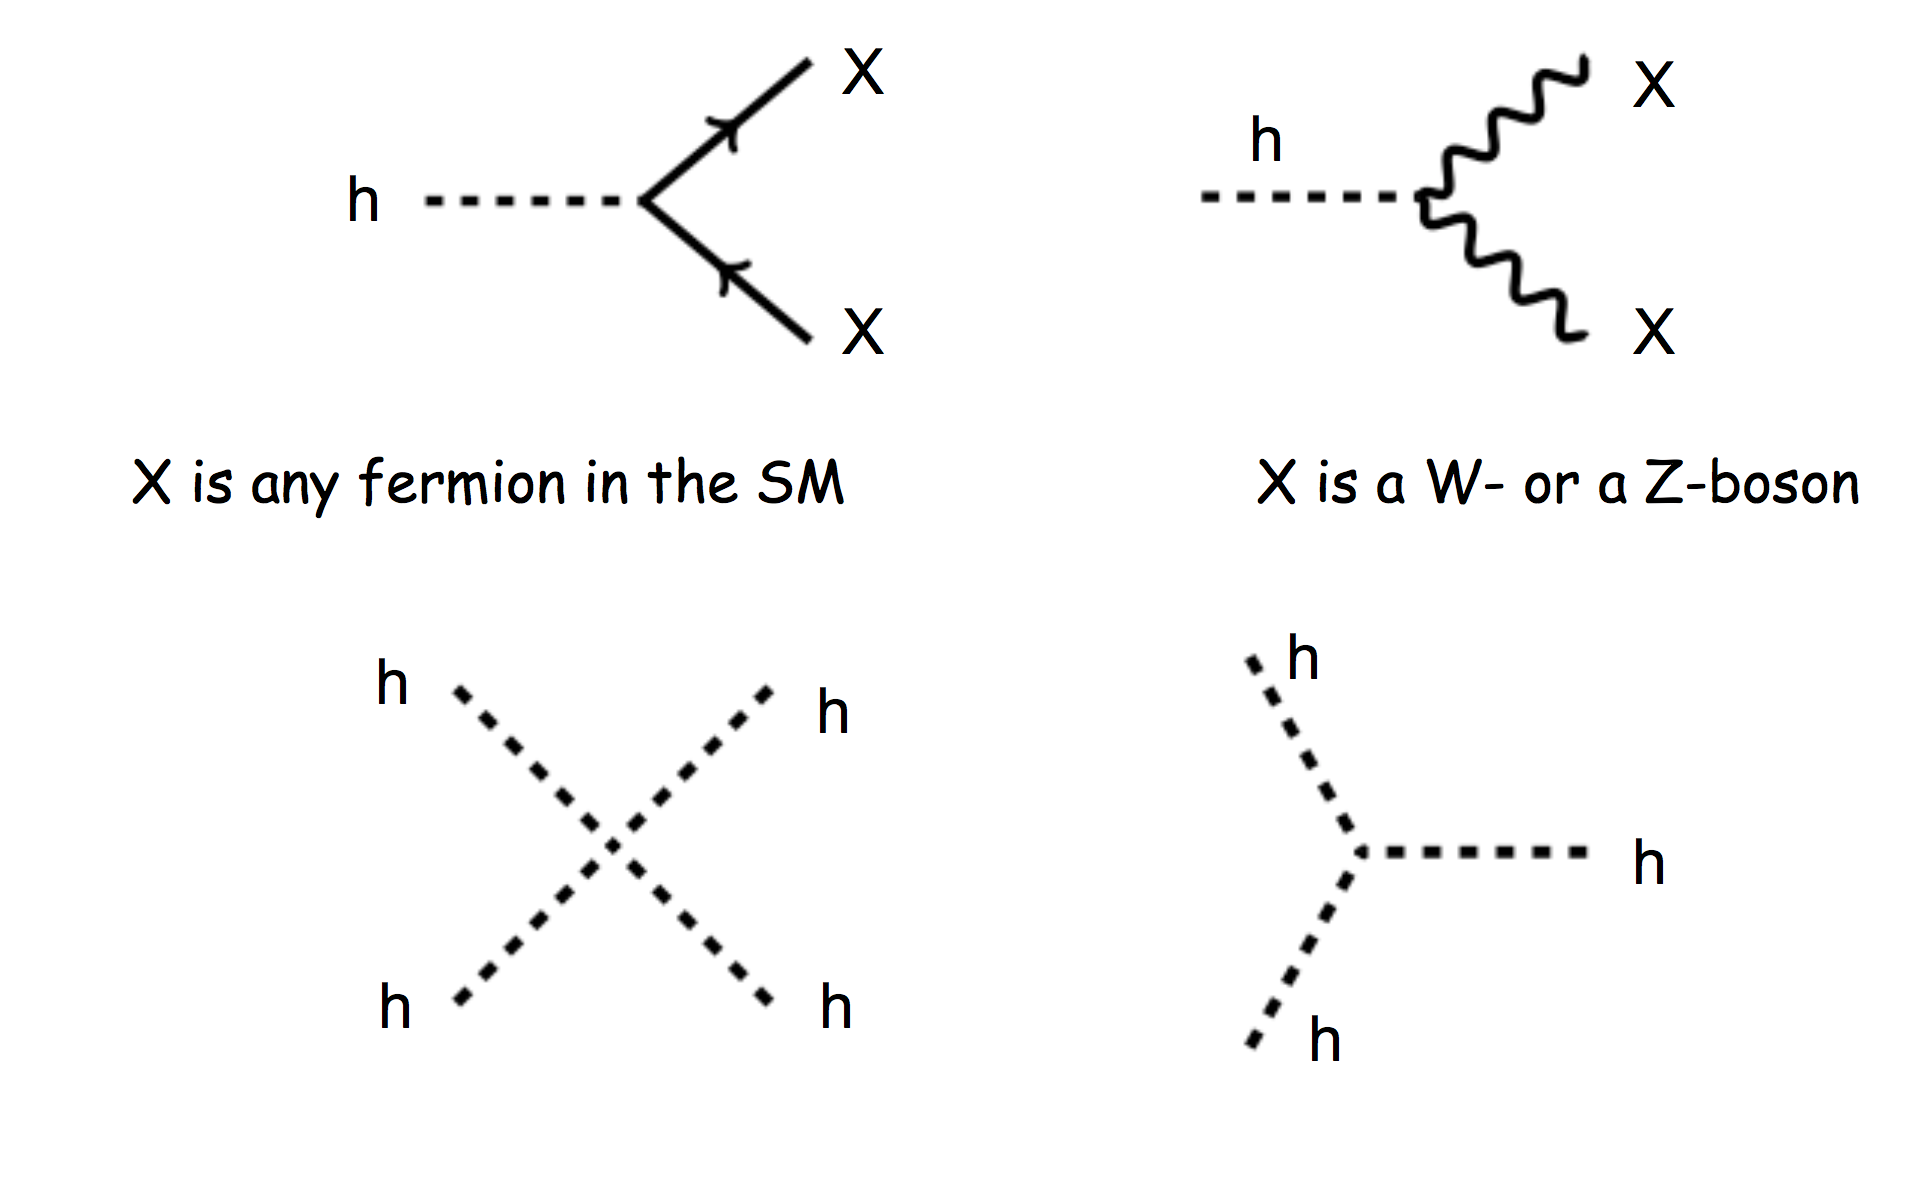
\includegraphics[width=\textwidth]{data/photo/theory/vertices_higgs.png}
\caption{All allowed fundamental higgs-related Feynman vertices in SM.}
\end{figure}
\end{column}

\end{columns}
\end{frame}

\end{document}
